\documentclass[a4paper,10pt]{article}

\usepackage[english]{babel}
\usepackage[utf8]{inputenc}
\usepackage{graphicx}
\usepackage[tbtags]{amsmath}
\usepackage{amssymb}
\usepackage{amsbsy}
\usepackage{eucal}
\usepackage{hyperref, url}
\usepackage{float}
\usepackage{verbatim} % For verbatiminput.
\usepackage{fancyvrb}
\usepackage{afterpage}

\pdfinfo{            
          /Title      (T-61.3050 Machine Learning: Basic Principles)
          /Author     ()
          /Keywords   ()
}

\DefineVerbatimEnvironment {code}{Verbatim}
   {%numbers=left,numbersep=2mm,
     %frame=lines,framerule=0.1mm, 
     fontsize=\small}
\RecustomVerbatimCommand{\VerbatimInput}{VerbatimInput}
   {%numbers=left,numbersep=2mm,
     frame=lines,framerule=0.1mm, fontsize=\small}
\DefineVerbatimEnvironment {outputlog}{Verbatim}
  {frame=lines,framerule=0.1mm, fontsize=\small}

\newcommand{\XXX}[1]{{\bf XXX #1}}
\parindent 0mm
\parskip 3mm

%------------------------------------------------------------------------------
% First page
%------------------------------------------------------------------------------

% add your student number in parenthesis
\title{T-61.3050 Term Project, final report\\ % Dictated in instructions.
       Using decision trees for spam classification}
\author{Jori Bomanson (81819F) \\
  {\tt jori.bomanson@aalto.fi} \\
  \\
  Sami J. Lehtinen (44814P)\\ 
  {\tt sjl@iki.fi} \\
}
\begin{document}

\floatstyle{plain}
\newfloat{Listing}{t}{lol}
\floatname{Listing}{Listing}

\maketitle
\thispagestyle{empty}
\pagebreak
\pagenumbering{arabic}

\section{Abstract}
% Include the key points of your work in a few sentences (including methods
% used and conclusions).
We trained a univariate binary classification tree to detect email spam.


\section{Rationale}

The choice of using a decision tree to solve a task with boolean variables
seemed natural. Such a tree could definitely match whatever complexity there
would be in the training data.
In fact we figured our success would be determined mainly by how we would
manage to avoid overfitting.

Decision trees were also tempting in that they are much easier to
visualize than, e.g., naive bayes classifiers.  For example, see
figure \ref{fig:prune-both-pruned-6000}.

One reason to study decision trees was that we assumed many groups would
take on naive bayesian classifiers, and we wanted to do something a bit
different.

\section{Principles of decision trees}

Decision trees are a non-parametric method for data classification.
They don't try to approximate any model behind the data, instead relying
on a tactic of ``similar inputs produce similar outputs''.

\XXX{description and pseudo-code for the algorithm}

\subsection{Calculating impurity}

We chose to measure impurity with the entropy function
\cite[p. 176]{alpaydin2004}\footnote{Alpaydin cites ``(Quinlan 1986)''
  for the impurity algorithm.}.

\begin{equation*}
\begin{split}
\mathcal{I}_m &= - \sum_{i=1}^K p_m^i \log_2 p_m^i  \\
\text{for a node} \quad & m  \\
\text{where} \quad 0 \log 0 &\equiv 0  \\
p_m^i &= P(\text{Instance reaching node m belongs to class i})  \\
K &= 2
\end{split}
\end{equation*}

\subsection{Pruning the tree}

Decision trees can be trained to perfectly match the training
data\cite[p. 182]{alpaydin2004}.  This will lead the model to
gross overfitting, which manifests as a large generalization error.
This can be avoided by pruning the tree.  There are two non-exclusive
approaches to pruning, prepruning and postpruning.

Without pruning, a tree with a training set size of 1000 looks like
figure \ref{fig:no-pruning-1000}.

\begin{figure}[h]
  \centering
  \begin{minipage}[c]{1.0\textwidth}
    \centering
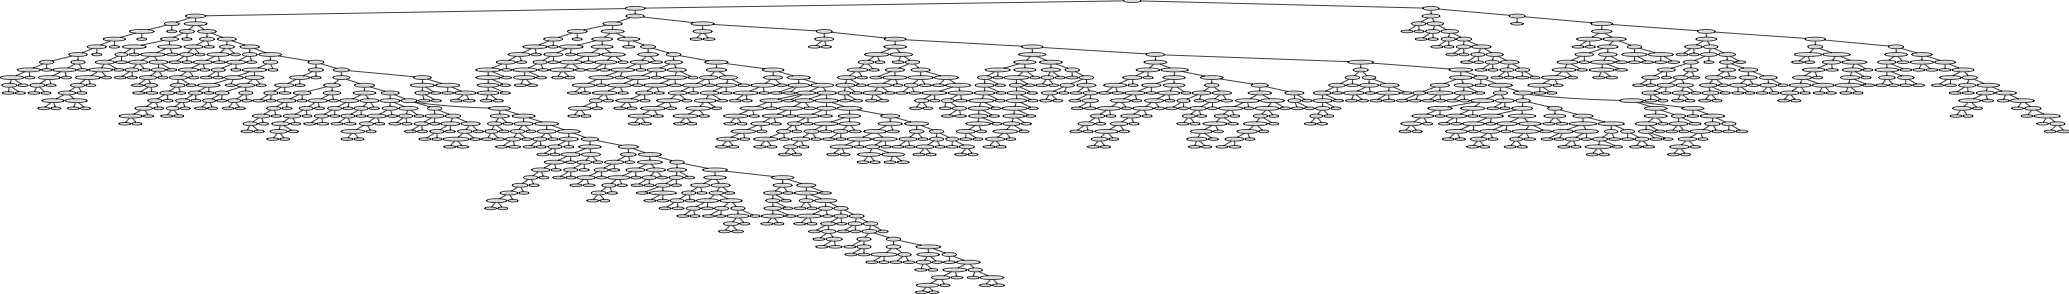
\includegraphics[width=130mm]{no-pruning-1000.png}
  \end{minipage}
  \caption{Tree from training set of 1000 elements, that hasn't been
    pruned.}
  \label{fig:no-pruning-1000}
\end{figure}

Still, against the test set the non-pruned tree faired surprisingly
well, achieving an accuracy of over 94 percent.

% \begin{verbatim}
% Classified as spam: 5556 / 9000
% Validation:
%  Classified as spam: 5556 / 9000
%  Classified as spam in validation set: 5989 / 9000
%  Correctly classified: 8499
%  Correctly classified as spam: 5522
%  Accuracy: 0.944
%  Precision: 0.994
%  Recall: 0.922
%  Perplexity: 1.324
% \end{verbatim}

\subsubsection{Prepruning}

In prepruning, the recursion of the training algorithm is stopped once
certain limits are reached.  Examples include impurity and number of
data rows.

In our first versions of the classifier we only did prepruning, which
resulted in very small and tidy trees, but the accuracy left comething
to be desired (94-95 percent).  We used one of the suggested
approaches from \cite{alpaydin2004}, where we make the tree as pure as
possible (no prepruning) and handle overfitting by postpruning the tree.

Removing prepruning didn't have an adverse effect for the final
accuracy, indeed, accuracy increased by a couple percentage points with
a large training set (6000).  The complexity of the tree is dramatically
increased as a side effect, though; where a pre- and postpruned tree,
trained with 6000 elements, has 59 nodes, the tree that was not
prepruned contains nearly 7000 nodes.  Training time is also a lot
longer without prepruning, which makes sense, given how many extra nodes
are introduced.

\begin{figure}
  \centering
\begin{tabular}{|l|c|c|c|c|}
\hline
 & Accuracy & Precision & Recall & Perplexity \\ \hline
1000, not pruned &  0.944 & 0.994 & 0.922 & 1.324 \\
1000, pre & 0.953 & 0.987 & 0.941 & 1.268 \\
1000, post & 0.953 & 0.984 &  0.944 & 1.182 \\
1000, pre + post &  0.955 & 0.984 & 0.947 & 1.201 \\
\hline
\end{tabular}
  \caption{Effects of pruning on accuracy and other characteristics,
    1000 training data points.}
  \label{fig:pruning} 
\end{figure}

\begin{figure}
  \centering
\begin{tabular}{|l|c|c|c|c|}
\hline
 & Accuracy & Precision & Recall & Perplexity \\ \hline
6000, pre + post & 0.973 & 0.983 & 0.975 & 1.130 \\
6000, post & 0.977 & 0.991 & 0.974 & 1.178 \\
\hline
\end{tabular}
  \caption{Effects of pruning on accuracy and other characteristics,
    6000 training data points.}
  \label{fig:pruning6000} 
\end{figure}


\begin{figure}
  \centering
\begin{tabular}{|l|c|c|c|c|}
\hline
 & Training time in seconds \\ \hline
6000, pre + post & 869 \\
6000, post & 3694 \\
\hline
\end{tabular}
\caption{Effects of pruning on training time 6000 training data points.}
  \label{fig:pruning6000-training-time} 
\end{figure}

%Pre- and postpruned, 1000 items.
%
%\begin{verbatim}
%Classified as spam: 5744 / 9000
%Validation:
% Classified as spam: 5744 / 9000
% Classified as spam in validation set: 5966 / 9000
% Correctly classified: 8594
% Correctly classified as spam: 5652
% Accuracy: 0.955
% Precision: 0.984
% Recall: 0.947
% Perplexity: 1.201
%\end{verbatim}

When prepruning, we stopped the algorithm by limiting by the results
from the entropy calculation, by columns (features) and rows (messages)
left in a recursion step.  For example, \XXX{more detailed explanation}.

1000 items in training set, theta = 0.04, min\_row\_ratio = 0.002

\begin{figure}[h]
  \centering
  \begin{minipage}[c]{1.0\textwidth}
    \centering
\includegraphics[width=130mm]{prepruned-1000.pdf}
  \end{minipage}
  \caption{Prepruned tree from a training set of 1000 elements.}
  \label{fig:prepruned-1000}
\end{figure}

%Prepruned, 1000 items.
%\begin{verbatim}
%Validation:
% Classified as spam: 5684 / 9000
% Classified as spam in validation set: 5962 / 9000
% Correctly classified: 8578
% Correctly classified as spam: 5612
% Accuracy: 0.953
% Precision: 0.987
% Recall: 0.941
% Perplexity: 1.268
%\end{verbatim}

\subsubsection{Postpruning}
\label{sect:postpruning}

Postpruning is used to reduce generalization error by using a a special
pruning data set to check whether removing a subtree from the decision
tree will result in the same or smaller error against the pruning set.

\begin{figure}[h]
  \centering
  \begin{minipage}[c]{1.0\textwidth}
    \centering

\includegraphics[width=130mm]{prune-both-original-6000.pdf}
  \end{minipage}
  \caption{Prepruned tree from a training set of 6000 elements.}
  \label{fig:prune-both-original-6000}
\end{figure}

\begin{figure}[h]
  \centering
  \begin{minipage}[c]{1.0\textwidth}
    \centering

\includegraphics[width=130mm]{prune-both-pruned-6000.pdf}
  \end{minipage}
  \caption{Pre- and postpruned tree from a training set of 6000 elements.}
  \label{fig:prune-both-pruned-6000}
\end{figure}

\XXX{table of errors with a postpruned tree}
\begin{figure}[h]
  \centering
  \begin{minipage}[c]{1.0\textwidth}
    \centering
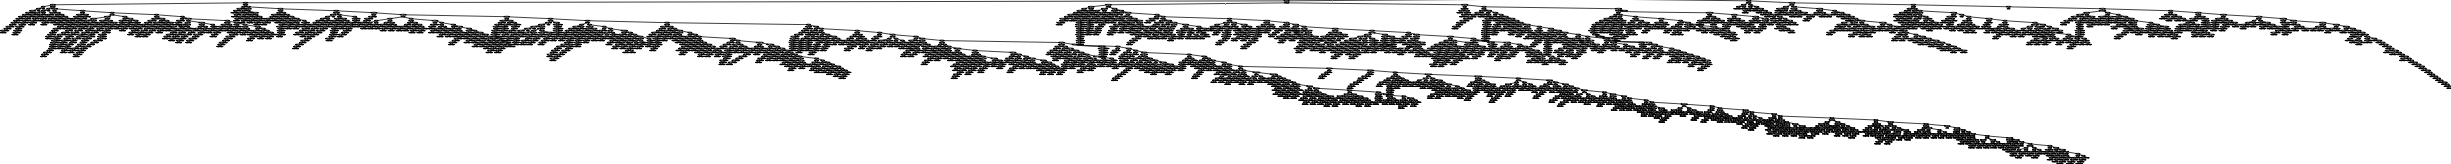
\includegraphics[width=130mm]{postpruned-pruned-6000.png}
  \end{minipage}
  \caption{Postpruned tree from a training set of 6000 elements.}
  \label{fig:no-pruning-6000}
\end{figure}

% Postpruned, 1000 items.
% \begin{verbatim}
% 1000 items.
% Chosen classifier has accuracy of 0.98.
% Classified as spam: 5709 / 9000
% Validation:
%  Classified as spam: 5709 / 9000
%  Classified as spam in validation set: 5952 / 9000
%  Correctly classified: 8579
%  Correctly classified as spam: 5620
%  Accuracy: 0.953
%  Precision: 0.984
%  Recall: 0.944
%  Perplexity: 1.182
% \end{verbatim}

% \begin{verbatim}
% 6000 items, pre- and postpruning.
% Validation:
%  Classified as spam: 2604 / 4000
%  Classified as spam in validation set: 2626 / 4000
%  Correctly classified: 3890
%  Correctly classified as spam: 2560
%  Accuracy: 0.973
%  Precision: 0.983
%  Recall: 0.975
%  Perplexity: 1.130
% \end{verbatim}

% \begin{verbatim}
% 6000 items, just postpruning.
% Validation:
%  Classified as spam: 2601 / 4000
%  Classified as spam in validation set: 2648 / 4000
%  Correctly classified: 3907
%  Correctly classified as spam: 2578
%  Accuracy: 0.977
%  Precision: 0.991
%  Recall: 0.974
%  Perplexity: 1.178
% \end{verbatim}
% \begin{verbatim}
% real	61m33.824s
% user	57m22.444s
% sys	1m15.947s
% \end{verbatim}

It should be noted that training the set without prepruning takes many
times longer than with it.

Prepruned tree takes a hit in accuracy, but is much faster to train.

% \begin{verbatim}
% Validation:
%  Classified as spam: 2608 / 4000
%  Classified as spam in validation set: 2683 / 4000
%  Correctly classified: 3881
%  Correctly classified as spam: 2586
%  Accuracy: 0.970
%  Precision: 0.992
%  Recall: 0.964
%  Perplexity: 1.233
% 
% real	14m28.909s
% user	12m18.457s
% sys	1m18.402s
% \end{verbatim}

\section{Validation of our approach}

\subsection{Accuracy, precision, recall, and perplexity}

The criteria for measuring the goodness of the classifier are the same
as the ones used in the data challenge.  As described in
\cite{termproject}, accuracy is the fraction of test set messages
classified correctly.  The precision is the ratio of correctly
classified spam messages to all messages classified as spam.  Recall is
the ratio of correctly classified spam messages to all spam messages.

Perplexity is calculated with

\begin{equation}
P = \exp(-\operatorname{mean}(\ln{Pi}))
\end{equation}

where $Pi$ is the probability of the email message being of the correct
class.

For the perplexity calculation, we return the probability that a message
is spam based on the ratio of spam messages left at the leaf node that
ends up deciding whether the message is spam or not.  This seems a
decent metric for calculating perplexity, at least when comparing to
what other groups reported in the data challenge.

\subsection{K-fold cross validation}

We implemented 10-fold cross validation to our classifier.  This
gave more stable values for generalization error when compared to
repeatedly training the classifier without the cross validation.

One part of the training data set was used for postpruning the tree, see
section \ref{sect:postpruning}.

\subsection{Dummy model}


\section{Results with different training set sizes}

XXX results to a table.
\begin{figure}
  \centering
\begin{tabular}{|l|c|c|}
\hline
Tr. size & Training time & Accuracy \\ \hline
1000 & 44 & 0.942 \\
4000 & 581 & 0.966 \\
6000 & 1180 & 0.972 \\
\hline
\end{tabular}
  \caption{Effects of training set size, postpruned.}
  \label{fig:training-data-size} 
\end{figure}

% 1000 items.
% 
% \begin{verbatim}
% Chosen classifier has accuracy of 1.0.
% Classified as spam: 5777 / 9000
% Validation:
%  Classified as spam: 5777 / 9000
%  Classified as spam in validation set: 6134 / 9000
%  Correctly classified: 8475
%  Correctly classified as spam: 5693
%  Accuracy: 0.942
%  Precision: 0.985
%  Recall: 0.928
% 
% real	0m44.221s
% user	0m44.040s
% sys	0m0.150s
% \end{verbatim}
% 
% 4000 items in training set.
% 
% \begin{verbatim}
% Chosen classifier has accuracy of 0.9725.
% Classified as spam: 3984 / 6000
% Validation:
%  Classified as spam: 3984 / 6000
%  Classified as spam in validation set: 4064 / 6000
%  Correctly classified: 5798
%  Correctly classified as spam: 3923
%  Accuracy: 0.966
%  Precision: 0.985
%  Recall: 0.965
% 
% real	9m41.857s
% user	9m40.900s
% sys	0m0.520s
% \end{verbatim}
% 
% 6000 items in training set.
% 
% \begin{verbatim}
% Chosen classifier has accuracy of 0.978333333333.
% Classified as spam: 2677 / 4000
% Validation:
%  Classified as spam: 2677 / 4000
%  Classified as spam in validation set: 2725 / 4000
%  Correctly classified: 3886
%  Correctly classified as spam: 2644
%  Accuracy: 0.972
%  Precision: 0.988
%  Recall: 0.970
% 
% real	19m40.578s
% user	19m37.980s
% sys	0m1.100s
% \end{verbatim}

\subsection{Training algorithm complexity}

Base on figure \ref{fig:training-data-size}, training algorithm looks
strongly like a quadratic algorithm.  Training is much faster with
modest prepruning parameters, which decrease the tree size by a factor
of almost hundred.

\section{Conclusions}

The chosen approach didn't achieve the same high marks for accuracy as
the winners of the data challenge.  Tweaking of the approach is
naturally possible, but it seems that decision trees are more suited in
this as a part of combined classifier instead of on their own.  This
does not mean that the approach is completely without merits; decision
trees were applied here without prior knowledge to the distribution of
the spam messages.  In the data challenge, the winning teams had tweaked
the prior probabilities for spam to match the distribution in the data
set.  In the decision tree model, this is not necessary, or even
possible.

Looking at the generated decision trees, it is easy to follow the
process by eye (at least with the smaller trees).  This, we think, helps
a lot in validating the approach.

\section{Comments on project difficulty}

\begin{thebibliography}{9}
\bibitem{alpaydin2004}
  Ethem Alpaydin,
  \emph{Introduction to Machine Learning}.
  Massachusetts Institute of Technology, Cambridge, Massachusetts,
  1st edition,
  2004. 415 pages. ISBN 0-262-01211-1.
\bibitem{termproject}
  \emph{Term Project 2011: Spam or Ham?}.
  \href{https://noppa.aalto.fi/noppa/kurssi/t-61.3050/term\_project}
  {https://noppa.aalto.fi/noppa/kurssi/t-61.3050/term\_project}
  [Web article]. 2011-11-6. [Cited 2011-11-19].

%\bibitem{press07}
%  William H. Press, Saul A. Teukolsky, William T. Vetterling, Brian P. Flannery,
%  \emph{Numerical recipes - the art of scientific computing}.
%  Cambridge University Press, New York,
%  3rd edition,
%  2007. 1235 pages. ISBN 978-0-521-88068-8.
%\bibitem{mellin10a}
%  Ilkka Mellin, 
%  \emph{Todennäköisyyslaskenta ja tilastotiede: Kaavat}.
%  Otaniemi, 2010. 390 pages.
%\bibitem{mellin10b}
%  Ilkka Mellin, 
%  \emph{Tilastolliset taulukot}.
%  Otaniemi, 2010. 13 pages.
\end{thebibliography}

\afterpage{\clearpage} % Flush all floats so that they won't mingle with
                       % the python code, below.
\pagebreak
\appendix
\section{Python code for the classifier}

The code is also available at GitHub,
\href{https://github.com/sjlehtin/spam-or-ham/blob/master/decisiontree.py}
{https://github.com/sjlehtin/spam-or-ham/blob/master/decisiontree.py}.

\verbatiminput{decisiontree.py}

\end{document}
